\hypertarget{gptux4ee3ux7801ux5f00ux53d1ux548cux7f16ux5199ux4ee3ux7801}{%
  \section{GPT代码开发和编写代码}\label{gptux4ee3ux7801ux5f00ux53d1ux548cux7f16ux5199ux4ee3ux7801}}


在这个数字化时代,编程已经成为连接人类智慧与机器世界的桥梁。从智能手机到人工智能,每一行代码都在构建着我们未来的数字文明。但编程并非易事,它需要深奥的知识、严谨的逻辑和丰富的经验。

而GPT(生成式预训练变换模型)的出现,正在改变这一现状。这项革命性的技术不仅能够理解人类的语言,更能理解和生成高质量的代码。这不仅是技术创新的进步,更是人类智慧与机器智能融合的新起点。

本章将带您进入这个激动人心的技术领域,探索GPT如何成为每一位开发者的强大助力。无论您是编程新手还是经验丰富的开发者,都将在这里发现新的可能性,开启代码创作的新纪元。

\hypertarget{ux4f7fux7528gptux8fdbux884cux4ee3ux7801ux5f00ux53d1}{%
  \subsection{使用GPT进行代码开发}\label{ux4f7fux7528gptux8fdbux884cux4ee3ux7801ux5f00ux53d1}}

\hypertarget{ux80ccux666fux4e0eux6311ux6218}{%
  \subsubsection{背景与挑战}\label{ux80ccux666fux4e0eux6311ux6218}}

在传统的软件开发过程中,开发者需要面对一系列复杂的任务:

\begin{itemize}
  \item
        \textbf{需求理解}:将业务需求转化为技术实现
  \item
        \textbf{系统设计}:规划系统的架构和模块
  \item
        \textbf{编码实现}:编写高质量的代码
  \item
        \textbf{测试维护}:确保代码的稳定性和可维护性
\end{itemize}

这些环节不仅耗时耗力,还需要开发者具备跨领域的知识。GPT的出现为解决这些问题提供了新的思路。

\hypertarget{gptux5982ux4f55ux52a9ux529bux4ee3ux7801ux5f00ux53d1}{%
  \subsubsection{GPT如何助力代码开发}\label{gptux5982ux4f55ux52a9ux529bux4ee3ux7801ux5f00ux53d1}}

GPT通过以下方式改变传统的开发模式:

\begin{enumerate}
  \def\labelenumi{\arabic{enumi}.}
  \item
        \textbf{自动化生成文档}:根据现有代码自动生成API说明、用户手册
  \item
        \textbf{智能代码审查}:提供代码改进意见,发现潜在问题
  \item
        \textbf{快速原型开发}:根据需求描述快速生成初始代码框架
  \item
        \textbf{跨语言支持}:在不同编程语言之间进行转换和适配
\end{enumerate}

\hypertarget{ux4e3aux4ec0ux4e48ux9009ux62e9gpt}{%
  \subsubsection{为什么选择GPT?}\label{ux4e3aux4ec0ux4e48ux9009ux62e9gpt}}

\begin{enumerate}
  \def\labelenumi{\arabic{enumi}.}
  \item
        提高效率:减少重复性工作,加速开发流程
  \item
        增强质量:通过智能检查提升代码稳定性
  \item
        跨越鸿沟:连接业务需求与技术实现
  \item
        创新可能:探索传统方法难以触及的解决方案
\end{enumerate}

\hypertarget{ux5b9eux4f8bux6f14ux793agptux5728ux5f00ux53d1ux4e2dux7684ux5e94ux7528}{%
  \subsubsection{实例演示:GPT在开发中的应用}\label{ux5b9eux4f8bux6f14ux793agptux5728ux5f00ux53d1ux4e2dux7684ux5e94ux7528}}

\begin{enumerate}
  \def\labelenumi{\arabic{enumi}.}
  \item
        \textbf{生成API文档}

        \begin{itemize}
          \item
                输入代码片段,输出详细的接口说明:
        \end{itemize}

        \begin{lstlisting}
// 用户输入一段REST API的代码
GET /users
Response:
{
    "users": [
        {"id": 1, "name": "Alice"},
        {"id": 2, "name": "Bob"}
    ]
}

// GPT生成的API文档
### 用户管理接口

#### 获取用户列表
```http
GET /api/users
\end{lstlisting}

        响应格式

        \begin{lstlisting}
{
    "users": [
        {"id": number, "name": string}
    ]
}
\end{lstlisting}

        错误码

        \begin{itemize}
          \item
                401: 未认证
          \item
                500: 内部错误
          \item
                \ldots{}\ldots{}.
        \end{itemize}

  \item
        \textbf{代码审查与优化}

        \begin{lstlisting}
# 用户输入的原始代码
def calculate_average(numbers):
    sum = 0
    for number in numbers:
        sum += number
    average = sum / len(numbers)
    return average

# GPT建议的优化版本
def calculate_average(numbers):
    """计算数字列表的平均值"""
    if not numbers:
        return 0.0
    return sum(numbers) / len(numbers)
\end{lstlisting}
  \item
        \textbf{快速原型开发}

        \begin{itemize}
          \item
                用户需求描述:
                ``需要一个在线投票系统,用户可以创建投票、查看结果统计。''
          \item
                GPT生成的代码框架:

                \begin{lstlisting}
# models.py
class Poll(models.Model):
    title = models.CharField(max_length=200)
    description = models.TextField()
    created_at = models.DateTimeField(auto_now_add=True)
    votes = models.ManyToManyField(User, through='Vote')

class Vote(models.Model):
    user = models.ForeignKey(User, on_delete=models.CASCADE)
    poll = models.ForeignKey(Poll, on_delete=models.CASCADE)
    choice = models.CharField(max_length=200)

# views.py
@login_required
def create_poll(request):
    if request.method == 'POST':
        form = PollForm(request.POST)
        if form.is_valid():
            poll = form.save(commit=False)
            poll.created_by = request.user
            poll.save()
            return redirect('poll_list')
    else:
        form = PollForm()
    return render(request, 'create_poll.html', {'form': form})
\end{lstlisting}
        \end{itemize}
\end{enumerate}

\hypertarget{ux4f7fux7528gptux8fdbux884cux4ee3ux7801ux7f16ux5199}{%
  \subsection{使用GPT进行代码编写}\label{ux4f7fux7528gptux8fdbux884cux4ee3ux7801ux7f16ux5199}}

\hypertarget{ux80ccux666fux4e0eux6311ux6218-1}{%
  \subsubsection{背景与挑战}\label{ux80ccux666fux4e0eux6311ux6218-1}}

在日常编程中,开发者常常面临以下难题:

\begin{itemize}
  \item
        \textbf{语法错误}:拼写错误、括号不匹配等问题
  \item
        \textbf{逻辑问题}:算法实现、条件判断等复杂逻辑
  \item
        \textbf{风格统一}:保持代码的一致性和可读性
  \item
        \textbf{知识获取}:快速查找API、框架的使用方法
\end{itemize}

GPT通过强大的语义理解和生成能力,为这些问题提供了创新性的解决方案。

\hypertarget{gptux5982ux4f55ux63d0ux5347ux7f16ux7801ux6548ux7387}{%
  \subsubsection{GPT如何提升编码效率}\label{gptux5982ux4f55ux63d0ux5347ux7f16ux7801ux6548ux7387}}

\begin{enumerate}
  \def\labelenumi{\arabic{enumi}.}

  \item
        \textbf{智能代码补全}:根据上下文预测下一步代码
  \item
        \textbf{错误修正建议}:识别并提出修复方案
  \item
        \textbf{代码风格调整}:统一格式、优化命名
  \item
        \textbf{技术文档查找}:即时获取API说明和使用示例
\end{enumerate}

\hypertarget{ux4e3aux4ec0ux4e48ux9009ux62e9gpt-1}{%
  \subsubsection{为什么选择GPT?}\label{ux4e3aux4ec0ux4e48ux9009ux62e9gpt-1}}

\begin{enumerate}
  \def\labelenumi{\arabic{enumi}.}

  \item
        即时帮助:随时提供编程指导和建议
  \item
        提高质量:通过智能纠错提升代码可靠性
  \item
        节省时间:减少查找资料的时间成本
  \item
        创新思路:启发新的解决方案和实现方式
\end{enumerate}

\hypertarget{ux5b9eux4f8bux6f14ux793agptux5728ux7f16ux7801ux4e2dux7684ux5e94ux7528}{%
  \subsubsection{实例演示:GPT在编码中的应用}\label{ux5b9eux4f8bux6f14ux793agptux5728ux7f16ux7801ux4e2dux7684ux5e94ux7528}}

\begin{enumerate}
  \def\labelenumi{\arabic{enumi}.}
  \item
        \textbf{根据自然语言生成代码}

        \begin{itemize}
          \item
                用户输入:''我需要一个函数,可以计算两个数的和,并返回结果。''
          \item
                GPT生成代码:

                \begin{lstlisting}
def add_numbers(a, b):
    """Calculate the sum of two numbers."""
    return a + b
\end{lstlisting}


        \end{itemize}

  \item
        \textbf{修复语法错误}

        \begin{itemize}
          \item
                用户输入错误代码:

                \begin{lstlisting}
print("Hello World!)
\end{lstlisting}

                GPT检测到缺少引号,修正为:

                \begin{lstlisting}
print("Hello World!")
\end{lstlisting}
        \end{itemize}
  \item
        \textbf{优化代码逻辑}

        \begin{itemize}
          \item
                用户输入低效代码:

                \begin{lstlisting}
total = 0
for num in numbers:
    total += num
average = total / len(numbers)
\end{lstlisting}

                GPT建议更简洁的方式:

                \begin{lstlisting}
average = sum(numbers) / len(numbers) if numbers else 0
\end{lstlisting}
        \end{itemize}
  \item
        \textbf{代码风格统一}

        \begin{itemize}
          \item
                用户输入不一致的命名规范:

                \begin{lstlisting}
function getUserName(id) {
    return users[id].name;
}

function GetUserEmail(id) {
    return users[id].email;
}
\end{lstlisting}

                GPT调整为一致的驼峰式命名:

                \begin{lstlisting}
function getUserInfo(id, field) {
    return users[id][field];
}
\end{lstlisting}
        \end{itemize}
\end{enumerate}

\hypertarget{ux52a8ux624bux8bd5ux8bd5}{%
  \subsection{动手试试}\label{ux52a8ux624bux8bd5ux8bd5}}

在前面的介绍中,已经有了实例演示的例子,那么现在我们再尝试动手使用GPT写几个小例子吧\textasciitilde{}

正所谓古人云:``学而不思则罔,思而不学则殆''。

\hypertarget{ux6469ux65afux5bc6ux7801}{%
  \subsubsection{摩斯密码}\label{ux6469ux65afux5bc6ux7801}}

\begin{quote}
  摩尔斯电码(Morse
  code)也被称作摩斯密码,是一种时通时断的信号代码,通过不同的排列顺序来表达不同的英文字母、数字和标点符号。它发明于1837年,是一种早期的数字化通信形式。不同于现代化的数字通讯,摩尔斯电码只使用零和一两种状态的二进制代码,它的代码包括五种:短促的点信号``・'',保持一定时间的长信号``---'',表示点和划之间的停顿、每个词之间中等的停顿,以及句子之间长的停顿。
\end{quote}

各位读者肯定在众多影视作品中可以看到,那么现在我们就让GPT来完成一个这样的简单例子。

用户输入:``现在我想编写一个将自然语言转化为摩斯密码的代码,使用Python代码实现,就以''I
LIKE U``这个句子为例实现一下。''

GPT回复:

为了将自然语言句子转换为摩斯密码,我们可以按照以下步骤实现:

\begin{enumerate}
  \def\labelenumi{\arabic{enumi}.}
  \item
        \textbf{创建摩斯密码字典}:包含所有英文字母及其对应的摩斯码。
  \item
        \textbf{处理输入字符串}:将其转为大写,并去除非字母字符,分割成单词列表。
  \item
        \textbf{转换每个单词}:将每个字母转换为摩斯码,并用单个空格分隔。
  \item
        \textbf{合并单词间的摩斯码}:使用三个空格分隔不同单词。
\end{enumerate}

以下是完整的Python代码:

\begin{lstlisting}
# 创建摩斯密码字典
mos_codes = {
    'A': '.-', 'B': '-...', 'C': '-.-.', 'D': '-..', 'E': '.', 
    'F': '..-.', 'G': '--.', 'H': '....', 'I': '..', 'J': '.---', 
    'K': '-.-', 'L': '.-..', 'M': '--', 'N': '-.', 'O': '---', 
    'P': '.--.', 'Q': '--.-', 'R': '.-.', 'S': '...', 'T': '-', 
    'U': '..-', 'V': '...-', 'W': '.--', 'X': '-..-', 'Y': '-.--', 
    'Z': '--..'
}

# 获取输入并处理
input_str = input("请输入要转换的句子:").upper()
cleaned = ''.join([c if c in mos_codes or c == ' ' else '' for c in input_str])
words = cleaned.split()

# 转换为摩斯码
morse_words = []
for word in words:
    morse_word = [mos_codes[char] for char in word]
    morse_words.append(' '.join(morse_word))

# 合并单词之间的空格
final_morse = '   '.join(morse_words)
print(final_morse)
\end{lstlisting}

\textbf{示例输入输出:}

\begin{itemize}
  \item
        输入:``I LIKE U''
  \item
        输出:``.. .-.. .. -.- . ..-''
\end{itemize}

这段代码能够将输入句子转换为对应的摩斯密码,每个字母用单个空格分隔,单词之间用三个空格分隔。

通过我们本地运行,得到了正确的结果:

\centering
\begin{figure}[H] %H为当前位置,!htb为忽略美学标准,htbp为浮动图形
  \centering %图片居中
  
\includegraphics[width=0.7\textwidth]{assets/figures/image-20250210171257118.png} %插入图片,[]中设置图片大小,{}中是图片文件名
  \caption{摩斯密码输出} %最终文档中希望显示的图片标题
  \label{Fig.main1} %用于文内引用的标签
\end{figure}%结束环境

很有意思不是吗?现在你可以用摩斯密码对你想说的话进行加密了,你可以尝试继续让GPT改进,让这个简单代码不断完善并且可以处理中文相关的信息,动手试试看吧!

\hypertarget{ux607aux6492ux5bc6ux7801}{%
  \subsubsection{恺撒密码}\label{ux607aux6492ux5bc6ux7801}}

\begin{quote}
  \textbf{恺撒密码}(英语:Caesar
  cipher),或称\textbf{恺撒加密}、\textbf{恺撒变换}、\textbf{变换加密},是一种最简单且最广为人知的加密技术。它是一种替换加密的技术,明文中的所有字母都在字母表上向后(或向前)按照一个固定数目进行偏移后被替换成密文。例如,当偏移量是3的时候,所有的字母A将被替换成D,B变成E,以此类推。这个加密方法是以罗马共和时期恺撒的名字命名的,当年恺撒曾用此方法与其将军们进行联系。
\end{quote}

这次我们再尝试一个古典密码学中的经典加密,根据苏维托尼乌斯于公元二世纪写的《恺撒传》中的记载,恺撒曾用此方法对重要的军事信息进行加密,它的原理非常简单,就是将所有字母偏移固定的长度,就像下图:

\centering
\begin{figure}[H] %H为当前位置,!htb为忽略美学标准,htbp为浮动图形
  \centering %图片居中
  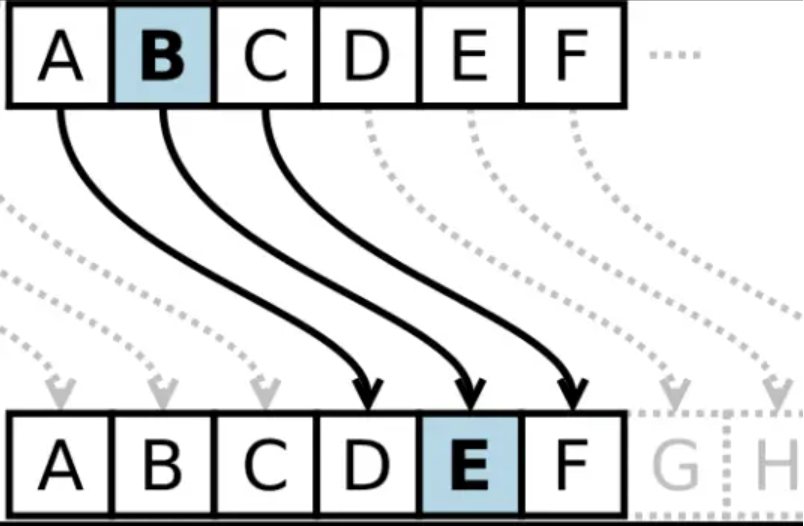
\includegraphics[width=0.7\textwidth]{assets/figures/image-20250210174403824.png} %插入图片,[]中设置图片大小,{}中是图片文件名
  \caption{恺撒加密示意图} %最终文档中希望显示的图片标题
  \label{Fig.main1} %用于文内引用的标签
\end{figure}%结束环境

那么现在我们同样用GPT来实现一个这样简单的例子:

用户输入:
``现在我想编写一个将自然语言转化为恺撒密码的代码,偏移量为3,使用Python代码实现,就以\texttt{My\ Fault\ forgive\ me\ for\ saying\ I\ like\ you\ here}这个句子为例实现一下。''

GPT回复:
好的!凯撒密码是一种替换加密技术,每个字母在字母表上向后移动固定的位数(这里是3位)。例如,`A'会被转换为'D',`B'会变成'E',依此类推。对于字母表的末尾字母(如'X'、`Y'、`Z'),它们会循环回到字母表的开头。

以下是将自然语言转化为凯撒密码的Python代码实现:

\begin{lstlisting}
def caesar_cipher(text, shift=3):
    result = []
    for c in text:
        if c.isupper():
            # 处理大写字母
            new_char = chr((ord(c) - ord('A') + shift) % 26 + ord('A'))
            result.append(new_char)
        elif c.islower():
            # 处理小写字母
            new_char = chr((ord(c) - ord('a') + shift) % 26 + ord('a'))
            result.append(new_char)
        else:
            # 非字母字符保持不变
            result.append(c)
    return ''.join(result)

# 示例句子
sentence = "My Fault forgive me for saying I like you here"
encrypted_sentence = caesar_cipher(sentence, shift=3)
print("加密后的句子:", encrypted_sentence)
\end{lstlisting}

\textbf{代码解释:}

\begin{enumerate}
  \def\labelenumi{\arabic{enumi}.}

  \item
        \texttt{caesar\_cipher}函数接受两个参数:\texttt{text}(要加密的文本)和\texttt{shift}(偏移量,默认为3)。
  \item
        遍历输入文本中的每个字符。
  \item
        对于大写字母,计算其在字母表中的新位置,并将结果转换回字符。
  \item
        对于小写字母,同样进行处理。
  \item
        非字母字符(如空格、标点符号等)保持不变。
  \item
        将所有处理后的字符拼接成最终的加密字符串。
\end{enumerate}

\textbf{示例运行:}

输入句子:``My Fault forgive me for saying I like you here''
加密后的输出会是:``Pb Idxow irujlyh ph iru vdblqj L olnh brx khuh''

这个代码可以将任何自然语言文本转换为凯撒密码,适用于需要简单加密的场景。

通过我们本地运行,得到了正确的结果:

\centering
\begin{figure}[H] %H为当前位置,!htb为忽略美学标准,htbp为浮动图形
  \centering %图片居中
  
\includegraphics[width=0.7\textwidth]{assets/figures/image-20250210173814654.png} %插入图片,[]中设置图片大小,{}中是图片文件名
  \caption{恺撒加密输出图} %最终文档中希望显示的图片标题
  \label{Fig.main1} %用于文内引用的标签
\end{figure}%结束环境

Eulooldqw!(Brilliant!)现在你可以用恺撒密码对你想说的话进行加密了,你可以尝试继续让GPT改进,让它可以解密恺撒密码,动手试试看吧!